\documentclass[fleqn,11pt]{SelfArx} % Document font size and equations flushed left

\setlength{\columnsep}{0.55cm} % Distance between the two columns of text
\setlength{\fboxrule}{0.75pt} % Width of the border around the abstract

\definecolor{color1}{RGB}{0,0,90} % Color of the article title and sections
\definecolor{color2}{RGB}{0,20,20} % Color of the boxes behind the abstract and headings

\newlength{\tocsep} 
\setlength\tocsep{1.5pc} % Sets the indentation of the sections in the table of contents
\setcounter{tocdepth}{3} % Show only three levels in the table of contents section: sections, subsections and subsubsections

%------------------------------------------------------------------------------------------------------------------------------------
%	ARTICLE INFORMATION
%------------------------------------------------------------------------------------------------------------------------------------

\JournalInfo{\ } % Journal information
\Archive{\ } % Additional notes (e.g. copyright, DOI, review/research article)

\PaperTitle{Advanced Computer Architecture: The ``Smooth'' Challenge} % Article title

\Authors{Romain Brault\textsuperscript{1}, Alexandre Camus\textsuperscript{2},  Giorgos Flourentzos\textsuperscript{3}} % Authors

\affiliation{\textsuperscript{1}RB812 \hfill \textsuperscript{2}AC5612 \hfill \textsuperscript{3}GF210}

\Keywords{} % Keywords - if you don't want any simply remove all the text between the curly brackets
\newcommand{\keywordname}{} % Defines the keywords heading name

%------------------------------------------------------------------------------------------------------------------------------------
%	USEFULL TOOLS
%------------------------------------------------------------------------------------------------------------------------------------

\usepackage[T1]{fontenc}
\usepackage[utf8]{inputenc}

\usepackage[english]{babel}

\usepackage{amsmath}
\usepackage{amsfonts}
\usepackage{amssymb}
\usepackage{amsthm}

\theoremstyle{definition}
\newtheorem{theorem}{Theorem}

\usepackage{enumerate}
\usepackage{caption}
\usepackage{subcaption}
\usepackage{listings}
\usepackage[pdftex=true,hyperindex=true,colorlinks=false,hidelinks]{hyperref}

\usepackage{tabularx}
\usepackage[lined,boxed,algonl]{algorithm2e}

\usepackage{etex}
\usepackage{tikz}
\usepackage{pgfplots}

\usepackage{placeins}

% Fonts packages (if needed)
%\usepackage[nott,fullsumlimits]{kpfonts}
%\usepackage{lmodern}
\renewcommand{\ttdefault}{txtt}

\usepackage{cite}

%------------------------------------------------------------------------------------------------------------------------------------
%	ABSTRACT
%------------------------------------------------------------------------------------------------------------------------------------

\Abstract{Coding is a question of how to compute things, but also how to compute them the fastest. These are often two questions that can't be resolved at once. Although coding a program that gives the expected result is an obstacle, another problem arises when performance is to be maximized. Once this is done, optimizing the written code might take a lot of time, depending on whether the hardware on which it is running, is taken into account. Here, given a correct program, the aim was to optimize it, given a chosen architecture. This consisted of understanding the code, then optimizing it sequentially and finally trying to improve it by parallelizing through vectorization or offloading the calculation to an accelerator (GPU).}

% ----------------------------------------------------------------------------------------------------------------------------------

\begin{document}


%------------------------------------------------------------------------------------------------------------------------------------
%	LISTINGS OPTIONS
%------------------------------------------------------------------------------------------------------------------------------------

\lstset{
basicstyle=\ttfamily,
keywordstyle=\color{blue},
identifierstyle=,
commentstyle=\color[rgb]{.2,.4,.5},
stringstyle=\ttfamily\color{gray},
breaklines=true,
language=c++}

%------------------------------------------------------------------------------------------------------------------------------------

\flushbottom % Makes all text pages the same height

\maketitle % Print the title and abstract box

\tableofcontents % Print the contents section

\thispagestyle{empty} % Removes page numbering from the first page

%------------------------------------------------------------------------------------------------------------------------------------

\section{Introduction}
\subsection{Context and Objectives}

Simulation in computer science is usually computationally intensive. Although an algorithm can be theoretically efficient\footnote{With a low complexity.}, an unoptimized implementation, without any hardware consideration reveals to be slower than expected.

This paper starts with a study of a basic implementation of a curve smoothing algorithm where the curve --- a mesh --- is represented by a graph. It presents various methods to reduce the computation time of the smoothing algorithm on a specific machine, according to the hardware specifications. The list of optimizations presented is non-exhaustive, however the considered approach reduced the computation time by approximately 1300\% on the given architecture.

The method used to achieve this speed-up is the following:
\begin{itemize}  \vspace{-4mm}
\item first optimize on one CPU core, \vspace{-4mm}
\item then parallelize over one node (here a single computer), \vspace{-4mm}
\item eventually use a hardware accelerator such as a GPU.
\end{itemize}

\subsection{Software Considerations}

The hardware considered is one of the Imperial College computing laboratory. All these computers are equipped with an Intel CPU, thus the best performance is obtained using the Intel Compiler\footnote{The speed-up gained by switching from g++ (GNU) to icpc (Intel) is presented in section \ref{seq}.}. However the Imperial College computers do not have the latest version of the Intel Compiler installed; providing some optimizations and the use of the new C++ standard (C++11). To obtain the maximum throughput an additional library not installed on Imperial College computers --- Blitz++ --- was used. In order to use the latest software available, the source code was compiled on a personal laptop which featured the latest Intel compiler version and the needed library. Then the executable was deployed on the target machine; this process being called Cross Compiling. To aid the cross compiling step the original makefile was generated through a CMake script.

Cross-compiling is challenging because the compiler usually tunes the code to be as fast as possible on the machine where the code is compiled, lowering the performance on the target machine. Extra care must be paid to the binary portability of the code. The code was compiled on a Linux-Fedora 18 64bits computer and is to run on a Linux-Ubuntu 12.04 64bits computer.


\FloatBarrier
\subsection{Hardware Considerations}

Tables \ref{CPUspecC} and \ref{CPUspecR} show respectively the hardware characteristics of the build machine and the target machine. The build machine is much slower than the target machine but is able to generate code optimized for the target machine.

\begin{table}[!h]
	\centering

	\begin{tabularx}{0.477\textwidth}{|m{3.5cm}|>{\raggedleft\arraybackslash}m{4cm}|}
		\hline
		Model Name & Intel Core i7-QM720 \\
		\hline
		Clock Speed & 1.6 GHz \\
		\hline
		Max Turbo Frequency & 2.8 GHz \\
		\hline
		Cache line size and alignment & 64 B \\
		\hline
		CPU cores & 4 \\
		\hline
		CPU Threads & 8 \\
		\hline
		Integrated GPU & No \\
		\hline
		Memory Channels & 2 \\
		\hline
		Max Memory Bandwith & 21 GB/s \\
		\hline
		Flags & fpu, sse, sse2, sse3, ssse3, sse4\_1, sse4\_2 \\
		\hline
	\end{tabularx}

	\caption{CPU Specifications for the compiling station.}
	\label{CPUspecC}
\end{table}

\begin{table}[!h]
	\centering

	\begin{tabularx}{0.477\textwidth}{|m{3.5cm}|>{\raggedleft\arraybackslash}m{4cm}|}
		\hline
		Model Name & Intel Core i7-2600 \\
		\hline
		Clock Speed & 3.4 GHz \\
		\hline
		Max Turbo Frequency & 3.8 GHz \\
		\hline
		Cache line size and alignment & 64 B \\
		\hline
		CPU cores & 4 \\
		\hline
		CPU Threads & 8 \\
		\hline
		Integrated GPU & Intel HD Graphics 2000 \\
		\hline
		Memory Channels & 2 \\
		\hline
		Max Memory Bandwith & 21 GB/s \\
		\hline
		Flags & fpu, sse, sse2, sse3, ssse3, sse4\_1, sse4\_2, avx \\
		\hline
	\end{tabularx}

	\caption{CPU Specifications for the running station.}
	\label{CPUspecR}
\end{table}

\paragraph{}

Figures \ref{topoR} and \ref{topoC} give the hardware topology of the build machine the target machine. Both use an Intel i7 placed on one socket with almost the same topology; the only difference being the size of the L3 cache which is 8M on the target machine compared to 6M on the build machine. The other main advantage of the Imperial College computer over the build architecture is the presence of AVX instructions. Therefore all the optimizations to tune the code on the laptop should be efficient on the Imperial College computer, except that the laptop should generate a binary including AVX instructions. As a result the binary could not run on the laptop which has generated the code, but it will be more efficient on the target machine.

\begin{figure}
	\centering

	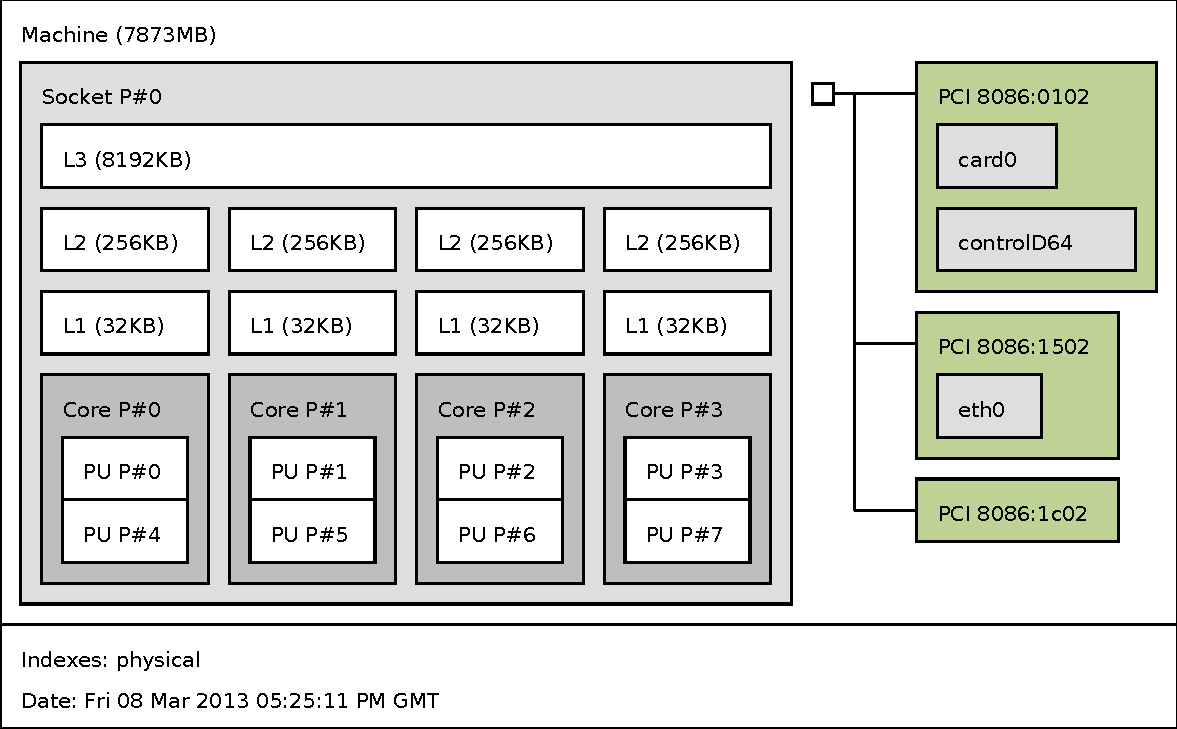
\includegraphics[width=.48\textwidth]{picture/run.pdf}

	\caption{Topology of the running station.}
	\label{topoR}
\end{figure}

\begin{figure}
	\centering

	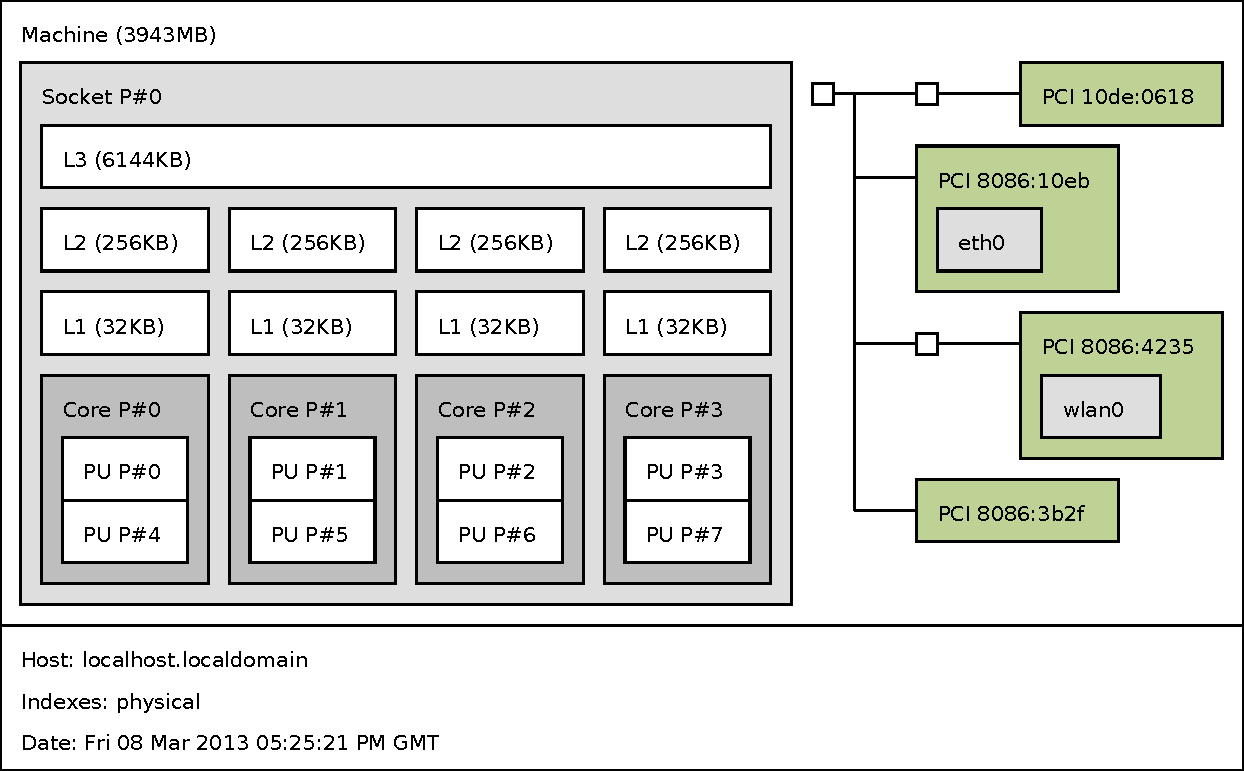
\includegraphics[width=.48\textwidth]{picture/compile.pdf}

	\caption{Topology of the compiling station.}
	\label{topoC}
\end{figure}


%------------------------------------------------------------------------------------------------------------------------------------
\FloatBarrier
\section{The Sequential Issue}
First the code was compiled with the g++ compiler, optimized at level 3, and analyzed with it Intel VTune Amplifier profiler to identify the bottlenecks. The initial run-time was $6.91$s for the small size graph, $54.0$s for the medium and $510$s for the large one. It appears that the initial program spent about 80\% of its time in the function \verb+mesh_quality()+. Hence that part of the code has been considered as a source of optimization.

A first approach to optimize the program was to change the compiler flags. The Intel profiler indicates that the program was spending a lot of time in computing square root and divisions. Thus a flag to reduce the precision of these operations has been set. Also when the code is split in multiple object files the compiler cannot optimize across these files, unless the flag "ipo" is set.

By reading the code, sequential issues were found. There are three kinds of problems: the source code structure, the algorithms chosen and the data representation.

\subsection{Source Code Structure}

A few changes in the structure of the code helped the compiler to optimize \verb+mesh_quality()+. Firstly, the code has been rewritten in order to be more object-oriented. All the attributes of the \verb+Mesh+ class have been set to private and the \verb+smooth+ function is now a method of this class. This did not really increase the performance but improved readability and maintainability. Additionally increasing the modularity of the code allows the compiler to do more optimizations as long as all the classes or functions are not spread across multiple files. It might also help the compiler to improve its generated code as it expects to process object-oriented code. 

Inline functions eliminate the overhead of function calls. Many small functions that frequently called in \verb+mesh_quality()+ and \verb+smooth()+ were good candidates for inlining. That is why functions as \verb+isSurfaceNode()+, \verb+isCornerNode()+, \verb+element_quality()+ or eventually \verb+svd_solve_2x2()+ were inlined.

In loops, changes have been made to avoid recomputation of the invariant (e.g. calling \verb+.size()+ in a loop). Instead, this invariant is now stored in a local variable.

\subsection{Algorithm}

The method used to solve the system of equations was too general to be efficient since the program needs only to solve systems of two equations in two unknowns. The Cramer's rule based on determinants is far more efficient in this case. It is defined as following:

\begin{theorem}
\hrule \vspace*{1pt}
Given an equations system $Ax = b$, where $A$ is a squared matrix of size $n$, and $x$ and $b$ two $n$-vertical vectors.

If $\det A \neq 0$ then the system has exactly one solution. Its solution is:
\[x_i = \dfrac{\det A_i}{\det A}\]
where $x = (x_1,\dots,x_i)^T$ and $A_i$ is the matrix formed by replacing the $i$-th column of $A$  by the column vector $b$. 

In this case ($2\times2$), the result is:
\begin{align*}
x_1 &= \dfrac{(b_1 \times a_{2,2}) - (b_2 \times a_{1,2})}{(a_{1,1} \times a_{2,2}) - (a_{2,1} \times a_{1,2})} \\
x_2 &= \dfrac{(a_{1,1} \times b_2) - (a_{2,1} \times b_1)}{(a_{1,1} \times a_{2,2}) - (a_{2,1} \times a_{1,2})}
\end{align*}
\hrule
\end{theorem}

The use of the function \verb+pow()+ proved to be too heavy in the method \verb+element_quality()+. Because the number of multiplications is known at compile time, the use of three multiplications is more efficient here, e.g. \verb+x*x*x+.

\subsection{Data Representation}

The data structure used to represent graphs --- an adjacency list --- is fine and the most efficient for the considered smoothing algorithm. However, the C++ structures used seem to be a little too big in this case. The original program used a vector of set to represent the adjacency lists. The notion of a set to represent the edges facilitate the edition and construction of the graph. However the graph structure remains unchanged during processing, thus the set was replaced by a vector after construction. A vector is a simpler data structure which reduce element access time.

Similarly, the number of nodes does not exceed $10^6$ for the large graph which is less than the maximum integer value represented by \verb+uint32_t+ instead of a \verb+size_t+. \verb+uint32_t+ is lighter\footnote{4 bytes vs 8 bytes.} and faster to manipulate and was therefore preferred.

Finally the type of the vectors \verb+normals+ and \verb+ENList+ was changed: the {Blitz++ library}\footnote{\url{http://blitz.sourceforge.net/}} provides useful array representations with performance comparable to Fortran implementations. After testing it on the different vectors in the program, it appears that the type \verb+blitz::Array+ of this library was more efficient for the vectors that are linearly accessed. \verb+normals+ and \verb+ENList+ have this property\footnote{The results of the sequential optimization are presented \ref{seq}.}.

%------------------------------------------------------------------------------------------------------------------------------------

\section{CPU Parallelization}

\subsection{Analysis}

After comprehensive experiments aimed at making the sequential code run as fast as possible the approach of parallelization was taken. For the given program three loops were candidates for parallelization. Usually the most outer loop is preferred but in this case dependencies inhibit the parallelization of this loop. Parallelizing a loop requires an important constant time to prepare the threads. The two most inner loops were therefore rejected because they are too small and called to many times to outweigh the burden of the parallel initialization. Eventually the middle loop iterating over nodes of the graph has been parallelized. However all the nodes cannot be inspected at the same time while running the program. To achieve that, the loop needs to be modified in order to cut the graph in groups of independent nodes. In order to group nodes in batches the graph must be colored. Then each color represents nodes that can be inspected at the same time because they are not adjacent.

Graph coloring is very expensive in terms of computation time. An implementation which strives to find the least amount of colors takes too much time, as the structure of the graph is unknown.

\subsection{Optimization}

A first try was realized with a very complex algorithm that colors a graph with the minimum number of colors needed. The time cost of coloring the graph with this algorithm was higher than the original total execution time (hundreds of minutes) and is not constant (it depends on the number of nodes).

\begin{algorithm}[!h]
\SetKwData{Left}{left}
\SetKwData{This}{this}
\SetKwData{Up}{up}
\SetKwFunction{Union}{Union}
\SetKwFunction{FindCompress}{FindCompress}
\SetKwInOut{Input}{input}
\SetKwInOut{Output}{output}
\caption{The \texttt{coloring} Algorithm.}

\Input{the graph $G$}
\Output{$C$ the array containing the colors}
\BlankLine

creating $C$, the output of size: number of node\;
intializing each element of $C$ to $-1$\;
\For{$i \leqslant \text{number of node}$}{
	$C[i] \leftarrow get\_colors( G[i] )$\;
}
\Return C\;

\label{coloring}
\end{algorithm}

The coloring algorithm finally chosen was very basic. This greedy implementation tries to color the graph without necessarily minimizing the number of colors. It succeeds in coloring the graphs with 4 or 5 colors. Algorithms \ref{coloring} and \ref{getcolors}, given in pseudocode, show the implementation of the greedy coloring algorithm.

\begin{algorithm}[!h]
\SetAlgoLined
\SetKwInOut{Input}{input}\SetKwInOut{Output}{output}

\Input{the array $A$ of all neighbours of one node}
\Output{return the color $C$ which is not used by other neighbours}
\BlankLine

$C := 0$\;
\While{}{
	\For{$i \leqslant \text{number of neighbours}$}{
		\If{$C = A[i]$}{$C := C + 1$\; \textbf{break}\;}
	}
	\If{$i = \text{number of neighbours}$}{\Return C\;}
}

\caption{The \texttt{get\_colors} Algorithm.}
\label{getcolors}
\end{algorithm}

Then the parallelization has been performed by adding a \verb+for+ loop on the colors before the loop that inspects all the nodes of the graph. The color of each node is compared to the current color. If they are different the node is skipped. The parallelization is then simply done on the loop that inspects all the nodes.

%------------------------------------------------------------------------------------------------------------------------------------

%\cleardoublepage
%\onecolumn

\section{Results}

\definecolor{colsmall}{HTML}{D7191C}
\definecolor{collarge}{HTML}{ABDDA4}
\definecolor{colmedium}{HTML}{2B83BA}

\subsection{Efficiency}
\label{seq}

In this section, the results based on the optimizations described before will be presented, followed by a brief discussion of their nature.

\begin{table}[!h]
	\centering
	
	\begin{tabular}{l|c|c|c}
		 & small & medium & large \\  
		\hline
		g++ no opt. & 509.59 & 54.018 & 6.9819 \\
		icpc no opt. & 240.66 & 25.352 & 3.2656 \\
		icpc opt. & 37.812 & 4.0604 & 0.51839 \\
		parallel opt. & 154.057 & 16.288 & 2.0347 \\
		icpc parallel opt. & 37.812 & 4.0604 & 0.51839 \\
	\end{tabular}
	
	\caption{Run time of different levels of optimizations.}
\end{table}

\begin{figure*}
	\centering
    
	\begin{tikzpicture}
	\begin{axis}[
		xbar stacked,
		legend style={
		    legend columns=4,
		    at={(0.5,-0.19)},
		    anchor=north,
		    draw=none
		},
		ytick=data,
		tick label style={font=\footnotesize},
		legend style={font=\footnotesize},
		label style={font=\footnotesize},
		width=0.9\textwidth,
		bar width=10mm,
		xlabel={Time in Seconds},
		yticklabels={icpc parallel opt., icpc opt., icpc no opt., g++ no opt.},
		xmin=0,
		xmax=520,
		area legend,
		y=12mm,
		enlarge y limits={abs=0.625},
	]
	\addplot[colsmall,fill=colsmall] coordinates
	{(0.51839,0) (2.0347,1) (3.2656,2) (6.9819,3) };
	\addplot[colmedium,fill=colmedium] coordinates
	{(3.54201,0) (14.253,1) (22.09,2) (47.0362,3)};
	\addplot[collarge,fill=collarge] coordinates
	{(33.230,0) (137.769,1) (212.05,2) (455.57,3)  };
	\legend{small.vtu,medium.vtu,large.vtu}
	\end{axis}
	\end{tikzpicture}
	
    \caption{Run time graph for different level of optimizations}
    \label{graph:EffOMP}
\end{figure*}

From the figure \ref{graph:EffOMP}, it is clear to deduce that the tools alone play an important role in the runtime of the program. The Intel compiler outperforms the corresponding GCC compilation of the given code. After the optimization of the sequential code, a further increase in performance is clearly visible. As previously discussed, this step involved refining the code in order to take advantage of faster matrix calculations, caching of intermediate values, inlining functions in order to reduce unnecessary function calls and altering the data structures used in order to streamline access time and data locality.

The largest performance however was gained by parallelizing execution using OpenMP. This has allowed for a further 4x boost in performance, for a cumulative 13x performance increase when compared to the original implementation and toolchain. The best result was obtained by having 8 threads running in parallel. In the figure below, a comparison of different levels of parallelism is made for the sake of completeness.

\FloatBarrier

\subsection{Parallel Considerations}

\begin{table}[!h]
	\centering
	
	\begin{tabular}{>{\raggedright\arraybackslash}m{2.3cm}|c|c|c}
		Number of OpenMP tasks & small & medium & large \\  \hline
		1 & 2.0347 & 16.288 & 154.057 \\
		2 & 1.0457 & 8.5758 & 79.154 \\
		4 & 0.55083 & 4.4787 & 42.104 \\
		8 & 0.51839 & 4.0604 & 37.812 \\
		16 & 0.81551 & 5.0838 & 43.458 \\
	\end{tabular}
	
	\caption{Run time table of smoothing the graph for different numbers of threads with (icpc parallel opt.)}
\end{table}

In search of the number of threads that would yield the best performance, a variety of numbers multiple of 2 were tested. It appears that when the number of threads is less than 8, the full power of the processor is not used. As the specification in table \ref{CPUspecR} suggests, in order to fully utilize the power of the processor, 8 threads must be used. This is because the processor consists of 4 hyperthreaded cores, where each can handle two threads at a time.

\begin{figure}[!h]
    \centering
    
    \begin{tikzpicture}
        \pgfplotsset{compat=1.5}
        \begin{loglogaxis}[
            log ticks with fixed point,
            log basis y=10,
            width=0.475\textwidth,
            ylabel={Run time (seconds).},
            xlabel={Number of OpenMP tasks ($n$).},
            xmin=1,
            xmax=16,
            ymin=0.5,
            ymax=180,
            xtick={1,2,4,8,16},
            legend entries={small.vtu, medium.vtu, large.vtu},
            legend cell align=left,
            legend style={
            		    legend columns=4,
            		    at={(0.5,-0.2)},
            		    anchor=north,
            		    draw=none
            		},
        ]
        \addplot[
            color=black, thick, mark=+
        ] table [
            x=proc, y=time1
        ] {./data/threads_against_time.txt};
        \addplot[
            color=red, thick, mark==+
        ] table [
            x=proc, y=time2
        ] {./data/threads_against_time.txt};
        \addplot+[
            color=blue, thick, mark=+
        ] table [
            x=proc, y=time3
        ] {./data/threads_against_time.txt};
        \end{loglogaxis}
    \end{tikzpicture}
    
    \caption{Run time graph for smoothing for different number of threads (icpc parallel opt.)}
    \label{graph:timeMPI}
\end{figure}

Using too many threads on the other hand can be equally disastrous, however, as this will incur additional cost in terms of context switching whilst at the same time providing no more parallelization.

Based on the graph shown above in \ref{graph:timeMPI}, a diagram plotting the efficiency of the different thread configurations is presented. Although slightly beyond the scope of this project, it is interesting enough to compare the best performance configuration against the most efficient configuration.

\begin{table}[!h]
	\centering
	
	\begin{tabular}{>{\raggedright\arraybackslash}m{2.3cm}|c|c|c}
		Number of OpenMP tasks & small & medium & large \\  \hline
		1 & 2.0347 & 16.288 & 154.057 \\
		2 & 1.0457 & 8.5758 & 79.154 \\
		4 & 0.55083 & 4.4787 & 42.104 \\
		8 & 0.51839 & 4.0604 & 37.812 \\
		16 & 0.81551 & 5.0838 & 43.458 \\
	\end{tabular}
	
	\caption{Run time table of smoothing the graph for different numbers of threads with (icpc parallel opt.)}
\end{table}

\subsection{Parallel Efficiency Considerations}

As was suggested by the graph in \ref{graph:timeMPI}, the best configuration purely in terms of performance is 8 threads. However, in terms of efficiency, the graph above suggests otherwise. It appears that the best configuration for efficiency is 4, and this must be attributed to the fact that the processor only has 4 cores. Despite the fact that hyperthreading is available which allows the maximum number of threads to be 8, the hyperthreaded threads share the same core and cache, which makes them sub-optimal when compared to threads running on individual cores.

\begin{table}[!h]
	\centering
	
	\begin{tabular}{>{\raggedright\arraybackslash}m{2.3cm}|c|c|c}
		Number of OpenMP tasks & small & medium & large \\
		\hline
		1 & 100\% & 100\% & 100\% \\
		2 & 97.29\% & 94.96\% & 97.31\% \\
		4 & 92.35\% & 90.92\% & 91.47\% \\
		8 & 49.06\% & 50.14\% & 50.93\% \\
		16 & 15.59\% & 20.02\% & 22.16\% \\
	\end{tabular}
	
	\caption{Efficiency for smoothing the graph for different number of threads with (icpc parallel opt.)}
\end{table}

\newpage

\section{Conclusion}

To summarize the main points of the experiment, it can be shown that good tools make room for a lot of improvement in performance, and the right choice of tools for the right architecture is very important. In addition, more efficient and well-designed code that targets a particular architecture can make a difference even when the code is to be run in a sequential manner. However, for a vast improvement parallelization is key. Performance is critical to large calculations and massive processing, but efficiency can be thought of being of equal importance as well. It is often the case that the best configuration for performance might not be the same for efficiency.

\begin{figure}
    \centering
    
    \begin{tikzpicture}
        \pgfplotsset{compat=1.5}
        \begin{semilogxaxis}[
            log ticks with fixed point,
            log basis y=10,
            width=0.475\textwidth,
            ylabel={Efficiency (\%).},
            xlabel={Number of OpenMP tasks ($n$).},
            xmin=1,
            xmax=16,
            ymin=15,
            ymax=110,
            xtick={1,2,4,8,16},
            legend entries={small.vtu, medium.vtu, large.vtu},
            legend cell align=left,
            legend style={
            		    legend columns=4,
            		    at={(0.5,-0.2)},
            		    anchor=north,
            		    draw=none
            		},
        ]
        \addplot[
            color=black, thick, mark=+
        ] table [
            x=proc, y=time1
        ] {./data/threads_against_efficiency.txt};
        \addplot[
            color=red, thick, mark==+
        ] table [
            x=proc, y=time2
        ] {./data/threads_against_efficiency.txt};
        \addplot+[
            color=blue, thick, mark=+
        ] table [
            x=proc, y=time3
        ] {./data/threads_against_efficiency.txt};
        \end{semilogxaxis}
    \end{tikzpicture}
    
    \caption{Efficiency graph for smoothing for different number of threads (icpc parallel opt.)}
    \label{graph:timeMPI2}
\end{figure}

\end{document}